\documentclass[12pt, hyperref={unicode}]{beamer}
\usepackage[utf8]{inputenc}
\usepackage[croatian]{babel}
\usepackage{multicol}
\usepackage{multirow}
\usepackage{graphicx}
\setbeamertemplate{footline}[frame number]
\setbeamertemplate{caption}[numbered]
\usetheme{Frankfurt}
\usecolortheme{beaver}

\title{Seminar iz kolegija Računalne vještine}
\subtitle{GitHub vs GitLab vs Bitbucket}
\author{Ivan Rubinić, Borna Sila, Mateo Srića}
\institute{Sveučilište u Rijeci - Tehnički fakultet}
\date{\today}

\begin{document}

\section{Naslovna strana}
\begin{frame}
	\titlepage
\end{frame}

%-------------------------------------------------------

\section{Uvod}
\begin{frame}
	\frametitle{Sadržaj prezentacije}
	\begin{columns}
		\column{0.55\textwidth}
			\tableofcontents
		\column{0.45\textwidth}
			\begin{figure}
			
\includegraphics
			[width = \linewidth]
			{slike/GitLab-vs-GitHub-vs-Bitbucket.jpg}
		\end{figure}
	\end{columns}
\end{frame}


\section{GitHub}
% \subsection{GitHub}
\begin{frame}[t]
	\frametitle{GitHub}
	\pause
	\setlength{\leftmargini}{0in}
	\begin{itemize}
		\item Web-baziran poslužiteljski servis koji služi za upravljanje inačicama koristeći Git\pause
		\item Koristi se za \textbf{dijeljenje i zajednički rad} na projektima\pause
		\item Koriste ga i velike kompanije kao \textbf{Google, IBM, Twitter, PayPal...}\pause
		\item Nude \textbf{besplatne, Pro, Team i Enterprise} račune\pause
	\end{itemize}
	\begin{figure}
		
\includegraphics
		[width = 0.7\linewidth]
		{slike/github-logo.png}
		\caption{GitHub logo}
	\end{figure}
\end{frame}


% \subsection{GitHub}
\begin{frame}[t]
	\frametitle{GitHub}
	\framesubtitle{Općenito}
	\pause
	\setlength{\leftmargini}{0in}
	\begin{itemize}
		\item Osnovan \textbf{2008.} godine\pause
		\item Djeluje sa sjedištem u \textbf{San Franciscu}\pause
		\item Matična organizacija - \textbf{Microsoft}\pause
		\item Osnivači GitHuba - \textbf{Tom Preston-Werner, Chris Wanstrath, Scott Chacon, P. J. Hyett}\pause
	\end{itemize}
	\begin{figure}
		
\includegraphics
		[width = 0.3\linewidth]
		{slike/github-cat.png}
		\caption{GitHub octocat}
	\end{figure}
\end{frame}

% \subsection{Povijest}
\begin{frame}[t]
	\frametitle{GitHub}
	\framesubtitle{Povijest}
	\setlength{\leftmargini}{0in}
	\begin{itemize}
		\begin{overprint}
			\onslide<2> \item Veljača 2008. - nastanak GitHuba
			\onslide<3> 
			\item Veljača 2008. - nastanak GitHuba 
			\item Do svibnja 2009. - više od 46000 javnih repozitorija i 100000 korisnika, do istog vremena sljedeće godine sadrži preko milijun repozitorija
			\onslide<4>
			\item Veljača 2008. - nastanak GitHuba 
			\item Do svibnja 2009. - više od 46000 javnih repozitorija i 100000 korisnika, do istog vremena sljedeće godine sadrži preko milijun repozitorija
			\item Polovicom 2011. - GitHub premašuje Google Code i SourceForge po broju commitova u proteklih šest mjeseci
			\onslide<5>
			\item Veljača 2008. - nastanak GitHuba 
			\item Do svibnja 2009. - više od 46000 javnih repozitorija i 100000 korisnika, do istog vremena sljedeće godine sadrži preko milijun repozitorija
			\item Polovicom 2011. - GitHub premašuje Google Code i SourceForge po broju commitova u proteklih šest mjeseci \item 2013. - milijun korisnika i 5 milijuna repozitorija
			\onslide<6>
			\item 2014. - 10 milijuna repozitorija
			\onslide<7>
			\item 2014. - 10 milijuna repozitorija
			\item 2016. - 14. mjesto na Forbesovoj listi Cloud 100
			\onslide<8>
			\item 2014. - 10 milijuna repozitorija
			\item 2016. - 14. mjesto na Forbesovoj listi Cloud 100
			\item 2018. - žrtva najvećeg DDoS napada u povijesti
			\onslide<9>
			\item 2014. - 10 milijuna repozitorija
			\item 2016. - 14. mjesto na Forbesovoj listi Cloud 100
			\item 2018. - žrtva najvećeg DDoS napada u povijesti
			\begin{figure}
			 	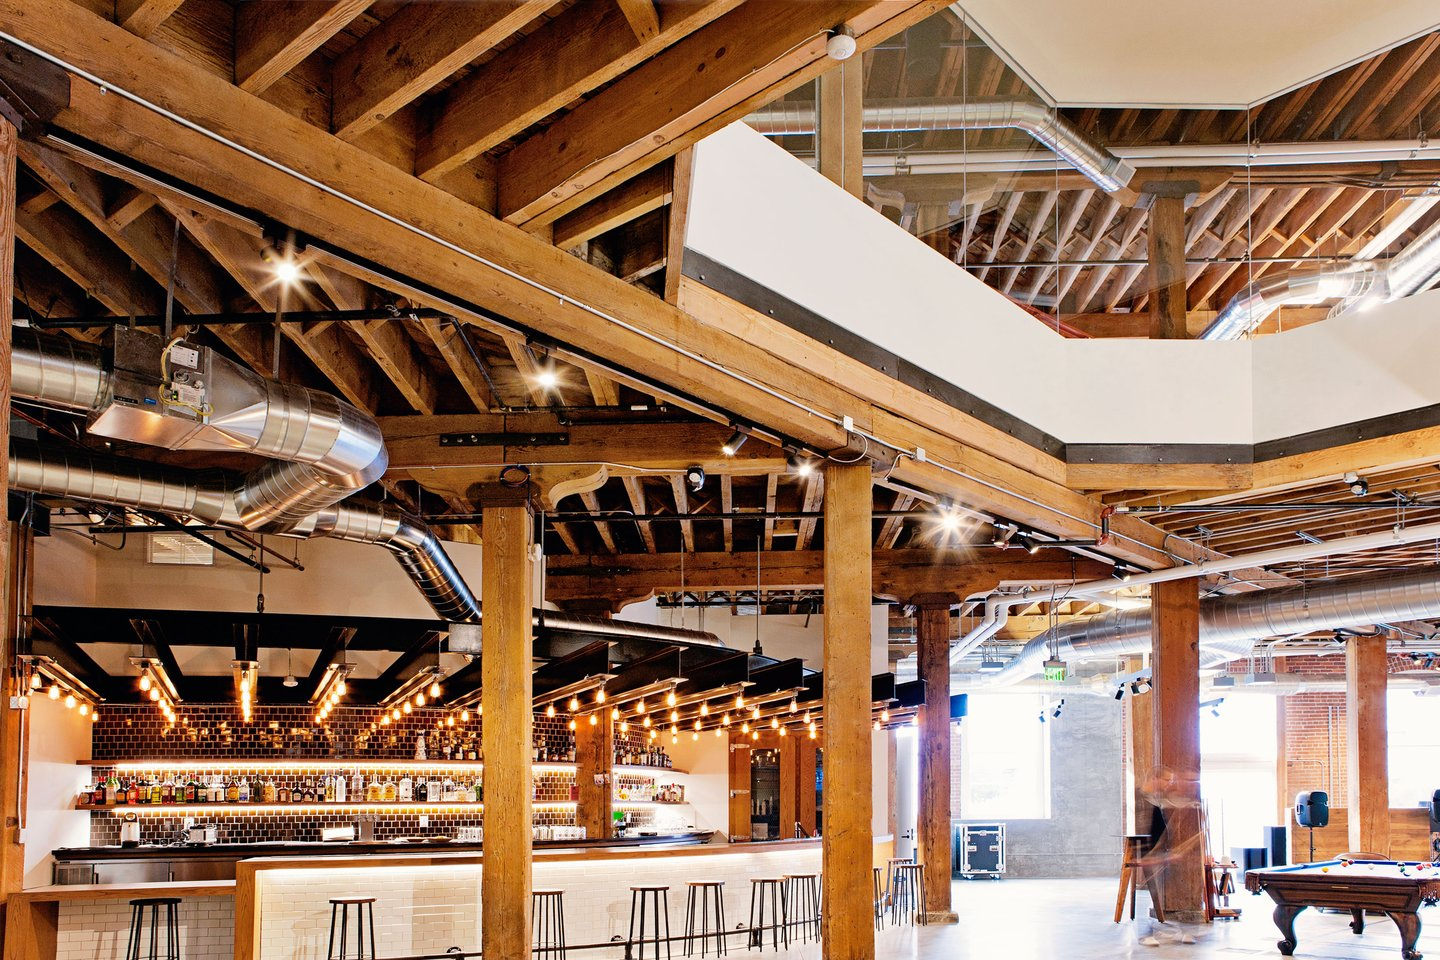
\includegraphics
			 	[width = 0.5\linewidth]
			 	{slike/github-hq.jpg}
			 	\caption{Unutrašnjost sjedišta GitHub-a}
			\end{figure}
		\end{overprint}
	\end{itemize}
\end{frame}

% \subsection{Pristup repozitorijima}
\begin{frame}[t]
	\frametitle{GitHub}
	\framesubtitle{Pristup repozitorijima}
	\setlength{\leftmargini}{0in}
	\pause
	\begin{itemize}
		\item Projektima se može pristupiti koristeći standardni Git command-line interface i sve ostale Git komande\pause
		\item GitHub dopušta pretraživanje javnih repozitorija i neregistriranim korisnicima, ali ne i doprinos (contributing) nekom projektu\pause
		\item Funkcije slične društvenim mrežama - followeri, feedovi i grafovi koji prikazuju rad developera\pause
	\end{itemize}
	\begin{figure}
	 	
\includegraphics
	 	[width = 0.5\linewidth]
	 	{slike/access-dg.jpg}
	\end{figure}
\end{frame}

% \subsection{Usluge}
\begin{frame}
	\frametitle{GitHub}
	\framesubtitle{Usluge}
	\setlength{\leftmargini}{0.1in}
	\pause
	\begin{enumerate}
		\item Markdown i njemu slični formati
		\begin{itemize}
			\item Dokumentacija, autmatski stvorena README datoteka...
		\end{itemize}
		\pause
		\item Praćenje problema (Issue tracking)
		\begin{itemize}
			\item Uključuje zahtjeve za feature, oznake...
		\end{itemize}
		\pause
		\item Wikis
		\pause
		\item Pull requests
		\begin{itemize}
			\item Sadrže pregled koda i komentare
		\end{itemize}
		\pause
		\item Povijest commitova
		\pause
		\item Grafovi o suradnicima, commitovima, članovima...
		\pause
		\item Gist
		\begin{itemize}
			\item Dijeljenje dijelova koda i ostalih informacija s drugima
		\end{itemize}
	\end{enumerate}
\end{frame}

% \subsection{Cjenik}
\begin{frame}[t]
	\frametitle{GitHub}
	\framesubtitle{Cjenik}
	\pause
	\begin{table}
		\footnotesize
		\begin{center}
		\caption{Cjenik GitHub-a}
		\begin{tabular}{|p{4cm}||p{5cm}|}
			\hline
			Mjesečna naknada & Opis \\
			\hline
			0 USD & neograničeni repozitoriji, issues, bug tracking, project management \\
			\hline
			7 USD & neograničen broj suradnika, napredni alati \\
			\hline
			9 USD/korisnik (za timove) & neograničen broj korisnika, team access kontrole, upravljanje korisnicima i projektom \\
			\hline
			21\$/korisnik & sve mogućnosti uključene u ostale opcije, 99.95\% uptime, pojednostavljeno upravljanje računima... \\
			\hline
		\end{tabular}
		\end{center}
	\end{table}
\end{frame}


% \subsection{Zanimljivosti}
\begin{frame}
	\frametitle{GitHub}
	\framesubtitle{Zanimljivosti}
	\setlength{\leftmargini}{0in}
	\pause
	\begin{itemize}
		\item GitHub ima oko 800 zaposlenika
		\pause
		\item Registrirano je više od 31 mililjun korisnika
		\pause
		\item Mjesečno GitHub posjeti preko 30 milijuna ljudi, od čega se 70\% nalazi izvan SAD-a, a 36\% unutar Europe
		\pause
		\item Projekti na GitHub-u su napisani u 337 različitih programskih jezika od kojih su najpopularniji JavaScript, Python i Java
		\pause
		\begin{figure}
	 		
\includegraphics
	 		[width = 0.7\linewidth]
	 		{slike/funfacts.jpg}
		\end{figure}
	\end{itemize}
\end{frame}

%-------------------------------------------------------


\section{GitLab}
% \subsection{GitLab}
\begin{frame}
	\frametitle{GitLab}
	\setlength{\leftmargini}{0in}
	\pause
	\begin{itemize}
		\item Sjedište također u \textbf{San Franciscu, SAD} \pause
		\item Open-core razvojni model \pause
	\end{itemize}
	\begin{figure}
	 	
\includegraphics
	 	[width = 0.5\linewidth]
	 	{slike/gitlab-logo.jpg}
	 	\caption{Logo GitLab-a}
	\end{figure}
\end{frame}

% \subsection{Povijest}
\begin{frame}[t]
	\frametitle{GitLab}
	\framesubtitle{Povijest}
	\setlength{\leftmargini}{0in}
	\begin{itemize}
		\begin{overprint}
			\onslide<2> \item Osnovao Sytse Sidbrandij i Dmitiriy Zaporozhets u 2013. godini
			\onslide<3> 
			\item Osnovao Sytse Sidbrandij i Dmitiriy Zaporozhets u 2013. godini
			\item Početna ideja : Dimitriy treba alat za suradnju sa svojim kolegama (open-source program)
			\onslide<4>
			\item Osnovao Sytse Sidbrandij i Dmitiriy Zaporozhets u 2013. godini 
			\item Početna ideja : Dimitriy treba alat za suradnju sa svojim kolegama (open-source program)
			\item Podjela na dvije verzije : CE-Community Edition i EE-Enterprise Edition
			\onslide<5>
			\item Osnovao Sytse Sidbrandij i Dmitiriy Zaporozhets u 2013. godini
			\item Početna ideja : Dimitriy treba alat za suradnju sa svojim kolegama (open-source program)
			\item Podjela na dvije verzije : CE-Community Edition i EE-Enterprise Edition
			\item Nove verzije programa izlaze mjesečno no EE postaje licencirana
			\onslide<6>
			\item Početni novac podiže više puta od raznih ulagača
			\onslide<7>
			\item Početni novac podiže više puta od raznih ulagača
			\item GNOME u svibnju 2018. godine prebaciju preko 400 projekata
			\onslide<8>
			\item Početni novac podiže više puta od raznih ulagača
			\item GNOME u svibnju 2018. godine prebaciju preko 400 projekata
			\item Kada je GitHub kupljen od strane Microsofta, mnogi pojekti su premješteni na GitLab
			\onslide<9>
			\item Početni novac podiže više puta od raznih ulagača
			\item GNOME u svibnju 2018. godine prebaciju preko 400 projekata
			\item Kada je GitHub kupljen od strane Microsofta, mnogi pojekti su premješteni na GitLab
			\item 11. kolovoza 2018. GitLab se prebacuje na Google Cloud platformu
		\end{overprint}
	\end{itemize}
\end{frame}

% \subsection{Cjenik}
\begin{frame}[t]
	\frametitle{GitLab}
	\framesubtitle{Cjenik}
	\pause
	\begin{table}
		\footnotesize
		\begin{center}
		\caption{Cjenik GitLab-a}
		\begin{tabular}{|p{4cm}||p{5cm}|}
			\hline
			Mjesečna naknada po članu & Opis \\
			\hline
			\textbf FREE & neograničeni repozitoriji i projekti uz potporu, issues, CI/CD \\
			\hline
			\textbf BRONZE 4\$ & + Code Quality, Merge approvals i podrška koja znatnije ubrzava razvoj programa \\
			\hline
			\textbf SILVER 19\$ & + grafovi \textit{pipeline} između projekata, Deploy Boards, Canars Deployments \\
			\hline
			\textbf GOLD 99\$ & sve usluge GitLaba \\
			\hline
		\end{tabular}
		\end{center}
	\end{table}
\end{frame}


% \subsection{Fun facts}
\begin{frame}
	\frametitle{GitLab}
	\framesubtitle{Zanimljivosti}
	\setlength{\leftmargini}{0in}
	\pause
	\begin{itemize}
		\item U siječnju 2017. godine, zbog posljedica napada, administrator je slučajno obrisao bazu podataka te je time 6 sati rada izgubljeno; oporavak se uživo prenosio preko www.youtube.com \pause
		\item Sjedište je u San Franciscu, a broj zaposjenih prelazi 400 i to u čak 41 zemlji i regiji \pause
		\item Preko 100000 organizacija koristi usluge GitLab-a: \textbf{Nasa, Sony, Electronic arts, Siemens...} \pause
		\begin{figure}
	 		
\includegraphics
	 		[width = 0.5\linewidth]
	 		{slike/funfacts.jpg}
		\end{figure}
	\end{itemize}
\end{frame}

\begin{frame}
	\frametitle{GitLab}
	\framesubtitle{Fun facts}
	\setlength{\leftmargini}{0in}
	\pause
		\begin{figure}
	 		
\includegraphics
	 		[width = 0.8\linewidth]
	 		{slike/companies.png}
	 		\caption{Organizacije koje koriste usluge GitLab-a}
		\end{figure}
\end{frame}
%-------------------------------------------------------

\section{Bitbucket}

% \subsection{Bitbucket}
\begin{frame}[t]
	\frametitle{Bitbucket}
	\framesubtitle{Općenito}
	\pause
	\setlength{\leftmargini}{0in}
	\begin{itemize}
		\item Web baziran poslužiteljski servis za pohranjivanje i upravljanjem različitih inačica istog projekta\pause
		\item Koristi \textbf{Mercurial} i \textbf{Git}\pause
		\item Koristi Mercurial od početka rada, Git tek od 2011.\pause
		\item 2016. - preko \textbf{5 milijuna} developera i \textbf{900 tisuća timova} na platformi\pause
	\end{itemize}
	\begin{figure}
		
\includegraphics
		[width = 0.7\linewidth]
		{slike/Bitbucket.png}
        \caption{Bitbucket logo}
	\end{figure}
\end{frame}


\begin{frame}[t]
	\frametitle{Bitbucket}
	\framesubtitle{Povijest}
	\pause
	\setlength{\leftmargini}{0in}
	\begin{itemize}
		\item Osnovao ga je Jesper Noehr \textbf{2008. godine}\pause
		\item Tvrtka \textbf{Atlassian} ga kupuje 29. rujna 2010. godine\pause
        \begin{figure}
			
\includegraphics
			[width = \linewidth]
			{slike/Atlassian.png}
        \end{figure}
        \begin{figure}
			
\includegraphics
			[width = 0.3\linewidth]
			{slike/Jesper.jpg}
        	\caption{Jesper Noehr}
		\end{figure}
	\end{itemize}
\end{frame}


\begin{frame}[t]
	\frametitle{Bitbucket}
	\framesubtitle{Servisi}
	\pause
	\setlength{\leftmargini}{0in}
	\begin{itemize}
		\item Markdown formati, dokumentacija\pause
		\item Praćenje problema\pause
		\item Wikis\pause
		\item Pull requests\pause
		\item Statične stranice na Bitbucket Cloudu s bitbucket.io domenom\pause
        \item \textbf{Bitbucket Server} \pause
	    \item Kombinacija Git servera  i web sučelja napisano u Javi i napravljeno u Apache Mavenu
	\end{itemize}
\end{frame}


\begin{frame}[t]
	\frametitle{Bitbucket}
	\framesubtitle{Besplatni računi}
	\pause
	\setlength{\leftmargini}{0in}
	\begin{itemize}
		\item Maksimalno 5 korisnika uz neograničen broj repozitorija \pause
		\item S akademskom email adresom, besplatan studentima i profesorima \pause            
	\end{itemize}
	\begin{figure}
		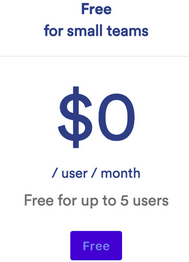
\includegraphics
		[width = 0.3\linewidth]
		{slike/free.png}
		\caption{Besplatni plan}
	\end{figure}
\end{frame}


\begin{frame}[t]
	\frametitle{Bitbucket}
	\framesubtitle{Plaćeni računi}
	\pause
	\setlength{\leftmargini}{0in}
	\begin{itemize}
		\item 10 korisnika za 10\$ mjesečno\pause
		\item 25, 50, 100 za 25\$, 50\$, 100\$ mjesečno\pause
		\item Neograničen broj korisnika za 200\$ mjesečno
	\end{itemize}
\end{frame}


\begin{frame}[t]
	\frametitle{Bitbucket}
	\framesubtitle{Plaćeni računi}
	\pause
	\setlength{\leftmargini}{0in}
	\begin{itemize}
		\item \textbf{Standard}\pause
            \begin{itemize}
				\item 2\$ po korisniku mjesečno s početnom vrijednosti od 10\$\pause
            \end{itemize}
        \item \textbf{Premium}\pause
            \begin{itemize}
	            \item 5\$ po korisniku mjesečno\pause
                \item Pristup dodatnim administrativnim značajkama kao \textbf{IP Whitelisting, Mirroring, Merge checks} i obavezna \textbf{2-step verifikacija} \pause
             \end{itemize}
	\end{itemize}
	\begin{figure}
		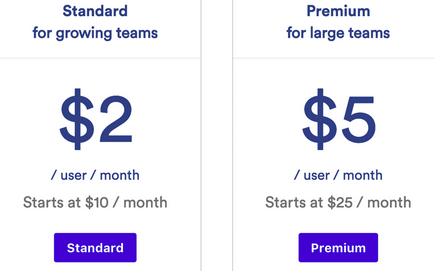
\includegraphics
		[width = 0.4\linewidth]
		{slike/standard-premium.png}
		\caption{Standard i Premium planovi}
	\end{figure}
\end{frame}

\section{GitHub vs GitLab vs Bitbucket}

\begin{frame}
	\frametitle{gh vs gl vs bb}
	\framesubtitle{Razlike}
	\pause
	\setlength{\leftmargini}{0in}
	\begin{itemize}
		\item Koriste različite izvore unosa repozitorija
		\item \textbf GitHub:\pause Git, SVN, HG, TFS
		\item \textbf Bitbucket:\pause Git, SVN, HG, CodePlex, Google Code 
		\item \textbf GitLab:\pause Git, drugi servisi: GitHub, Bitbucket, Google Code
	\end{itemize}
	\begin{figure}
		
\includegraphics
		[width = 0.5\linewidth]
		{slike/GitLab-vs-GitHub-vs-Bitbucket.jpg}
	\end{figure}
\end{frame}

\begin{frame}[t]
	\frametitle{gh vs gl vs bb}
	\framesubtitle{Razlike}
	\pause
	\begin{table}
		\footnotesize
		\begin{center}
		\caption{Cjenik GitHub-a}
		\begin{tabular}{|p{4cm}||p{5cm}|}
			\hline
			Naziv & Osnovano & Open source\\
			\hline
			GitHub & 2008. & NE \\
			\hline
			GitLab & 2008. Mercurial projekti; 2010./11. git hosting & DA \\
			\hline
			Bitbucket & 2012. pokrenuta; 2014. korporacija & otključana kupnjom verzije \\
			\hline
		\end{tabular}
		\end{center}
	\end{table}
\end{frame}

\begin{frame}[t]
	\frametitle{gh vs gl vs bb}
	\framesubtitle{Sličnosti}
	\setlength{\leftmargini}{0in}
	\begin{itemize}
		\begin{overprint}
			\onslide<2> \item lagano postavljanje
			\onslide<3> 
			\item lagano postavljanje 
			\item pull request i Code review
			\onslide<4>
			\item lagano postavljanje
			\item pull request i Code review
			\item Forks/clones repozitorija
			\onslide<5>
			\item lagano postavljanje 
			\item pull request i Code review
			\item Forks/clones repozitorija
			\item integracija programera treće strane (3rd party developers)
			\onslide<6>
			\item lagano postavljanje
			\item pull request i Code review
			\item Forks/clones repozitorija
			\item integracija programera treće strane (3rd party developers)
			\item snippets, Bug tracking
		\end{overprint}
	\end{itemize}
\end{frame}


\end{document}